\documentclass[11pt, a4paper]{article}

% ── Geometria ──────────────────────────────────────────────
\usepackage[a4paper, top=2.5cm, bottom=2.5cm, left=2cm, right=2cm]{geometry}

% ── Fonty & jazyk ──────────────────────────────────────────
\usepackage{fontspec}
\setmainfont{Noto Sans}
\usepackage{graphicx}
\usepackage[czech]{babel}

% ── Typografia ─────────────────────────────────────────────
\setlength{\parskip}{0.5em}
\setlength{\parindent}{0pt}

% ── Zoznamy ────────────────────────────────────────────────
\usepackage{enumitem}
\setlist[itemize]{label=--, itemsep=0.2em, topsep=0.3em, parsep=0pt}
\setlist[enumerate]{itemsep=0.25em, topsep=0.3em, parsep=0pt}

% ── Tabuľky ────────────────────────────────────────────────
\usepackage{booktabs}
\usepackage{tabularx}
\usepackage{array}

% ── Farby ──────────────────────────────────────────────────
\usepackage[table]{xcolor}
\definecolor{mainblue}{RGB}{0, 70, 127}
\definecolor{lightblue}{RGB}{220, 235, 252}
\definecolor{newblue}{RGB}{0, 100, 190}
\definecolor{darkgray}{RGB}{70, 70, 70}
\definecolor{ruleblue}{RGB}{120, 170, 220}

% ── TikZ ───────────────────────────────────────────────────
\usepackage{tikz}
\usetikzlibrary{arrows.meta, shapes.geometric}

% ── Nadpisy sekcií ─────────────────────────────────────────
\usepackage{titlesec}
\titleformat{\section}
  {\Large\bfseries\color{mainblue}}{\thesection}{0.8em}{}
  [\vspace{2pt}\color{ruleblue}\titlerule]
\titlespacing*{\section}{0pt}{1.4em}{0.8em}

\titleformat{\subsection}
  {\normalsize\bfseries\color{mainblue!85!black}}{\thesubsection}{0.6em}{}
\titlespacing*{\subsection}{0pt}{1em}{0.4em}

% ── Hlavička / Pätica ──────────────────────────────────────
\usepackage{fancyhdr}
\pagestyle{fancy}
\fancyhf{}
\fancyhead[L]{\small\color{darkgray}\textit{Platforma pro krátkodobé pronájmy nemovitostí}}
\fancyhead[R]{\small\color{darkgray}\textit{BUD0081 \textbar\ VAL0556 \textbar\ LIS0168}}
\fancyfoot[C]{\small\color{darkgray}\thepage}
\fancyfoot[R]{\small\color{darkgray}\textit{Ver.~0.2}}
\renewcommand{\headrulewidth}{0.4pt}
\renewcommand{\footrulewidth}{0.4pt}

% ── Hyperref ───────────────────────────────────────────────
\usepackage{hyperref}
\hypersetup{
    colorlinks=true,
    linkcolor=mainblue,
    urlcolor=mainblue,
    pdftitle={Semestrální projekt -- Platforma pro krátkodobé pronájmy nemovitostí},
}

% ============================================================
% VLASTNÉ PRÍKAZY
% ============================================================

% Nadpis podsekcie FURPS s farebným pruhom
\newcommand{\furpssec}[2]{%
  \vspace{0.45cm}%
  \noindent\colorbox{lightblue}{%
    \parbox{\dimexpr\textwidth-2\fboxsep\relax}{%
      \vspace{3pt}\hspace{4pt}%
      \textbf{\textcolor{mainblue}{#1}}\enskip%
      {\small\textcolor{darkgray}{\textit{(#2)}}}%
      \hspace{4pt}\vspace{3pt}%
    }%
  }\par\vspace{0.25cm}%
}

% Nadpis podsekcie (Aktéri, Ext. systémy)
\newcommand{\subsechead}[1]{%
  \vspace{0.35cm}%
  \noindent\textbf{\textcolor{mainblue!85!black}{#1}}\par%
  \vspace{0.1cm}%
}

% Blok parametrov scénára (tabular s vodorovnými čiarami)
\newenvironment{scenparams}{%
  \par\vspace{0.1cm}%
  \noindent{\color{ruleblue}\rule{\textwidth}{0.8pt}}\nopagebreak%
  \vspace{2pt}\par\nopagebreak%
  \begin{tabular}{@{}p{4.7cm}@{\hspace{0.1cm}}p{\dimexpr\textwidth-5.0cm\relax}@{}}%
}{%
  \end{tabular}%
  \par\vspace{-2pt}%
  \noindent{\color{ruleblue}\rule{\textwidth}{0.8pt}}%
  \vspace{0.35cm}%
}

% Skratka: jeden riadok parametra scénára
\newcommand{\sprow}[2]{\textbf{#1:} & #2 \\[3pt]}

% ============================================================
\begin{document}
% ============================================================

% ── TITULNÁ STRANA ─────────────────────────────────────────
\begin{titlepage}
  \thispagestyle{empty}
  \centering
  \vspace*{2.5cm}

  {\color{mainblue}\rule{\textwidth}{2.5pt}}
  \vspace{0.7cm}

  {\fontsize{26}{32}\selectfont\bfseries\color{mainblue}
    Platforma pro krátkodobé\\[0.4em] pronájmy nemovitostí}

  \vspace{0.5cm}
  {\color{ruleblue}\rule{\textwidth}{0.8pt}}
  \vspace{0.8cm}

  {\Large\color{darkgray} Semestrální projekt -- SWI}

  \vspace{3.5cm}

  \begin{flushleft}
    \large\color{darkgray}
    \textbf{\color{mainblue}Tým:}\\[0.6em]
    \begin{tabular}{@{}l@{\hskip 1.5cm}l@{}}
      Matúš Budoš      & \texttt{BUD0081} \\[0.3em]
      Kristián Válek   & \texttt{VAL0556} \\[0.3em]
      Vojtěch Lisztwan & \texttt{LIS0168} \\
    \end{tabular}
  \end{flushleft}

  \vfill
  {\color{ruleblue}\rule{\textwidth}{0.8pt}}
  \vspace{0.4cm}
  {\large\color{darkgray}\today}
\end{titlepage}

% ── HISTÓRIA VERZIÍ ────────────────────────────────────────
\thispagestyle{fancy}
\section*{\color{mainblue}História verzií dokumentu}
\addcontentsline{toc}{section}{História verzií dokumentu}

\noindent\small\textit{%
  \textcolor{newblue}{Modrá barva označuje nový obsah přidaný ve verzi~0.2.}}

\vspace{0.4cm}
\begin{tabularx}{\textwidth}{|l|X|c|}
  \hline
  \rowcolor{lightblue}
  \textbf{Dátum} & \textbf{Zmeny} & \textbf{Ver.} \\
  \hline
  10.03.2026
    & Prvé odovzdanie -- titulná strana, obsah, dôvod zavedenia, slovné zadanie,
      zoznam modulov, FURPS, kritické situácie, hranice systému, kontext prostredia,
      charakteristika aktérov, Use Case diagramy pre správu nemovitostí
      a rezervačný subsystém, scénáre 10.2 a 10.3.
    & 0.1 \\
  \hline
  \textcolor{newblue}{10.03.2026}
    & \textcolor{newblue}{Doplnenie histórie verzií. Vytvorenie Use Case diagramu
      (TikZ) pre modul správy identit. Doplnenie scénáru 10.1 (Registrácia nového
      užívateľa) vrátane rozhodovania, větvení a smyček. Doplnenie rozhodovacieho
      kroku do scénáru 10.2. Vizuálne a prezentačné vylepšenia dokumentu.}
    & \textcolor{newblue}{0.2} \\
  \hline
\end{tabularx}

\vspace{0.8cm}

% ── OBSAH ──────────────────────────────────────────────────
\tableofcontents
\newpage

% ============================================================
\section{Důvod a okolnosti zavedení řešení}
% ============================================================

Platforma vzniká z potřeby digitálně a efektivně propojit majitele volných nemovitostí s hosty, kteří hledají krátkodobé ubytování. Cílem je plně automatizovat, zjednodušit a zabezpečit celý proces pronájmu od prvotního vyhledání bytu, přes blokaci termínu, až po úspěšné zaplacení a následné hodnocení pobytu. Odstraněním manuálních kroků se snižuje chybovost a riziko překryvu rezervací.

% ============================================================
\section{Slovní zadání, popis projektu od zákazníka}
% ============================================================

\textit{Zákazník (investor) přichází s požadavkem na vývoj nové, moderní platformy pro zprostředkování krátkodobých pronájmů, která má konkurovat stávajícím řešením na trhu lepším uživatelským zážitkem a nižšími transakčními poplatky pro lokální trh.}

\textbf{Motivace a vize:}
Cílem projektu je vytvořit ucelený informační systém fungující jako oboustranné tržiště (marketplace). Na jedné straně stojí pronajímatelé, kterým systém musí poskytnout jednoduché rozhraní pro evidenci majetku, správu dostupnosti a cenotvorbu. Na straně druhé jsou hosté, kteří vyžadují rychlý a intuitivní způsob, jak najít ubytování podle svých preferencí (lokalita, termín, kapacita).

\textbf{Klíčové procesy (Core Business):}
Absolutním jádrem platformy je spolehlivý rezervační engine. Zákazník striktně vyžaduje plnou automatizaci procesu -- od okamžiku, kdy host klikne na tlačítko „Rezervovat", se systém musí postarat o dočasné uzamčení termínu, aby nedošlo k tzv. overbookingu (dvojí rezervaci stejného termínu). Následně musí proběhnout hladké předání zákazníka na externí platební bránu a po úspěšné transakci automatické potvrzení rezervace oběma stranám via e-mail.

\textbf{Očekávaný výstup:}
Systém musí být nasaditelný v cloudovém prostředí (24/7), musí obsahovat administrátorský panel pro řešení sporů a moderaci obsahu. Velký důraz je kladen na modul hodnocení, který buduje důvěru v rámci komunity. Dostupnost termínů se nesmí ukládat staticky pro každý den, ale musí být počítána dynamicky na základě existujících blokací a platných rezervací, což zajistí vysokou konzistenci dat.

% ============================================================
\section{Seznam modulů projektu a jejich významných atributů}
% ============================================================

Systém se skládá ze 6 logických celků s definovanými datovými strukturami a unikátní identifikací objektů.

\begin{enumerate}[leftmargin=*, label=\textbf{\arabic*.}]

  \item \textbf{\textcolor{mainblue}{Modul správy identit}}\\
    \textit{Objekt Uživatel:}
    \texttt{id}~(PK), \texttt{email}~(unikátní), \texttt{password\_hash},
    \texttt{jmeno}, \texttt{prijmeni},
    \texttt{role}~(Host\,/\,Pronajímatel\,/\,Administrátor).

  \item \textbf{\textcolor{mainblue}{Modul správy nemovitostí}}\\
    \textit{Objekt Nemovitost:}
    \texttt{id}~(PK), \texttt{owner\_id}~(FK), \texttt{nazev}, \texttt{popis},
    \texttt{lokalita}, \texttt{max\_kapacita}, \texttt{standardni\_cena\_noc}.\\
    \textit{Objekt Fotografie:}
    \texttt{id}~(PK), \texttt{property\_id}~(FK), \texttt{cesta\_k\_souboru}.\\
    \textit{Objekt Blokace:}
    \texttt{id}~(PK), \texttt{property\_id}~(FK),
    \texttt{datum\_od}, \texttt{datum\_do}, \texttt{duvod}.

  \item \textbf{\textcolor{mainblue}{Rezervační modul}}\\
    \textit{Objekt Rezervace:}
    \texttt{id}~(PK), \texttt{guest\_id}~(FK), \texttt{property\_id}~(FK),
    \texttt{datum\_zacatku}, \texttt{datum\_konce}, \texttt{celkova\_cena},
    \texttt{stav}~(Pending\,/\,Confirmed\,/\,Cancelled).

  \item \textbf{\textcolor{mainblue}{Platební modul}}\\
    \textit{Objekt Platba:}
    \texttt{id}~(PK), \texttt{reservation\_id}~(FK),
    \texttt{transakce\_brany\_id}~(unikátní), \texttt{castka},
    \texttt{stav\_platby}.

  \item \textbf{\textcolor{mainblue}{Modul hodnocení}}\\
    \textit{Objekt Recenze:}
    \texttt{id}~(PK), \texttt{reservation\_id}~(FK), \texttt{autor\_id}~(FK),
    \texttt{text}, \texttt{hvezdicky}~(1--5).

  \item \textbf{\textcolor{mainblue}{Administrátorský panel}}\\
    \textit{Objekt Log:}
    \texttt{id}~(PK), \texttt{akce}, \texttt{casove\_razitko},
    \texttt{admin\_id}.

\end{enumerate}

% ============================================================
\section{Systémové požadavky FURPS}
% ============================================================

\furpssec{a.\enspace Funkčnost}{Functionality -- F}
\begin{itemize}
  \item \textbf{Správa identit:} Systém musí umožňovat bezpečné zakládání uživatelských účtů s rozdělením rolí a autentizaci (přihlašování).
  \item \textbf{Správa nabídek:} Pronajímatelé musí mít možnost provádět CRUD operace nad svými nemovitostmi, nahrávat fotografie a definovat výjimky v kalendáři (např. blokace z důvodu malování).
  \item \textbf{Rezervační proces:} Systém musí umět dynamicky vyhledávat volné kapacity, dočasně uzamknout zvolený termín pro konkrétního uživatele a spravovat životní cyklus rezervace.
  \item \textbf{Platební integrace:} Plná integrace na externí platební bránu s automatickým zpracováním HTTP webhooků pro potvrzení transakcí.
\end{itemize}

\furpssec{b.\enspace Vhodnost k použití}{Usability -- U}
\begin{itemize}
  \item \textbf{Responzivní design (Mobile-first):} Klientská část aplikace musí být plně optimalizována pro mobilní telefony, odkud se očekává většina provozu.
  \item \textbf{Transparentnost cen:} Host musí před platbou vidět jasný rozpis ceny (počet nocí $\times$ cena za noc + případné poplatky).
  \item \textbf{Intuitivní kalendář:} Pronajímatelům musí být k dispozici vizuální kalendář pro správu dostupnosti a přehled obsazenosti.
  \item \textbf{Jasná zpětná vazba:} Systém musí poskytovat srozumitelné chybové hlášky, zejména při selhání platby nebo obsazení termínu.
\end{itemize}

\furpssec{c.\enspace Spolehlivost}{Reliability -- R}
\begin{itemize}
  \item \textbf{Integrita dat (Zamezení Overbookingu):} Rezervační logika musí využívat ACID transakce (pesimistické zamykání řádků), aby se nikdy nerezervoval stejný byt dvěma lidem.
  \item \textbf{Automatická obnova (Self-healing):} Nedokončené nebo nezaplacené rezervace musí systém pomocí CRON úloh automaticky stornovat a termíny uvolnit.
  \item \textbf{Bezpečnost dat (GDPR):} Osobní údaje a platební detaily musí být chráněny šifrováním hesel a HTTPS komunikací.
\end{itemize}

\furpssec{d.\enspace Výkon}{Performance -- P}
\begin{itemize}
  \item \textbf{Rychlost vyhledávání:} Odezva při složitém dotazování (filtrace + dynamický přepočet kalendáře) nesmí přesáhnout 2~sekundy.
  \item \textbf{Rychlost transakcí:} Dočasné uzamčení termínu musí proběhnout v řádu milisekund, aby se minimalizovalo okno pro race-condition.
  \item \textbf{Škálovatelnost:} Systém musí zvládnout nárazové špičky návštěvnosti (např. vyhledávání před Silvestrem nebo prázdninami).
\end{itemize}

\furpssec{e.\enspace Schopnost údržby}{Supportability -- S}
\begin{itemize}
  \item \textbf{Modulární architektura:} Logika musí být striktně oddělena do 6 popsaných modulů. Chyba v modulu hodnocení nesmí shodit proces rezervace.
  \item \textbf{Rozšiřitelnost API:} Komunikace s externími poskytovateli (platební brána, e-mail) musí být navržena přes Interfaces/Adapters -- změna poskytovatele (Stripe → GoPay) postačí vyřešit novým adaptérem.
  \item \textbf{Auditovatelnost:} Všechny kritické operace (rezervace, platba, zrušení, ban) musí být trvale zaznamenávány v systémovém logu.
\end{itemize}

% ============================================================
\section{Kritické situace}
% ============================================================

\begin{itemize}
  \item \textbf{Systémové -- Výpadek konektivity externí služby:}
    Host zaplatí, peníze se strhnou z jeho bankovního účtu, ale dojde k výpadku sítě a platforma nedostane webhook od platební brány o úspěšnosti transakce. Systém si tak myslí, že je rezervace nezaplacena, přestože peníze byly odečteny.

  \item \textbf{Aplikační -- Souběh transakcí (Race Condition):}
    Dva různí hosté mají otevřený stejný detail nemovitosti na velmi žádaný termín (např. Silvestr). Oba kliknou na „Rezervovat" ve stejnou vteřinu. Bez ošetření atomickým zámkem by systém mohl půjčit stejný byt dvěma lidem na stejný termín -- což je z pohledu byznysu i technicky nepřípustné.
\end{itemize}

% ============================================================
\section{Hranice systému}
% ============================================================

\begin{itemize}
  \item \textbf{Ideální scénář:}
    Pronajímatel vloží plnohodnotně vyplněnou nabídku. Host aplikuje filtry, ihned najde volnou nemovitost, provede rezervaci a okamžitě zaplatí kartou. Systém změní stav na „Potvrzeno", zapíše termín do kalendáře a rozešle potvrzovací e-maily. Pobyt proběhne bez problémů.

  \item \textbf{Hraničně řešitelný scénář:}
    Host si zarezervuje byt (termín na 15 minut zablokuje), ale v průběhu platby mu selže prohlížeč nebo záměrně okno zavře. Systém pomocí CRON úloh identifikuje nedokončenou rezervaci, automaticky ji stornuje a uvolní termín dalším uživatelům -- bez zásahu administrátora.

  \item \textbf{Situace, které systém nezvládne vyřešit:}
    Host přijede a fyzicky poškodí vybavení bytu. Software umožní zanechat záporné hodnocení a zablokovat účet hosta, ale fyzické vymáhání škody, pojišťovací řízení ani samotná oprava nespadají do kompetence tohoto informačního systému.
\end{itemize}

% ============================================================
\section{Kontext prostředí}
% ============================================================

Platforma funguje jako webová aplikace v cloudovém prostředí (24/7) a slouží jako prostředník (marketplace). Systém negeneruje vlastní obsah -- veškerá nabídka vzniká na straně pronajímatelů a poptávka na straně návštěvníků. Operuje v prostředí internetu s nutností zabezpečené komunikace (HTTPS) a striktním dodržováním nakládání s osobními údaji (GDPR).

% ============================================================
\section{Charakteristika aktérů a prostředí}
% ============================================================

\subsechead{a.\enspace Aktéři, uživatelé, role}
\begin{itemize}
  \item \textbf{Host (Návštěvník):} Vyhledává ubytování, provádí rezervace a platby, uděluje hodnocení.
  \item \textbf{Pronajímatel (Majitel nemovitosti):} Zakládá profily nemovitostí, nahrává fotky, definuje ceny a kalendář blokací.
  \item \textbf{Administrátor:} Řeší spory, ruší účty, moderuje nabídky a kontroluje systémové logy.
  \item \textbf{Systém (Časovač/CRON):} Autonomní vnitřní aktér spouštějící periodické čistící procesy (např. rušení nezaplacených rezervací).
\end{itemize}

\subsechead{b.\enspace Externí systémy}
\begin{itemize}
  \item \textbf{Platební brána:} Zpracovává platby z karet a vrací systému status transakce (webhook).
  \item \textbf{E-mailový server (SMTP/API):} Fyzicky doručuje notifikace a potvrzení do schránek uživatelů.
  \item \textbf{Mapové služby:} Validují GPS souřadnice a vizualizují lokality ubytování.
\end{itemize}

\newpage

% ============================================================
\section{Use case diagramy}
% ============================================================

Každý člen týmu analyzoval odlišnou část systému a vytvořil vlastní Use Case diagram. Celkem jsou pokryty 3 moduly s využitím vzťahov \texttt{<<include>>} a \texttt{<<extend>>}.

% ── UC 1: Správa identit (NOVÉ v 0.2) ──────────────────────
\subsection{\textcolor{newblue}{Modul správy identit (BUD0081)}}

{\color{newblue}
Diagram zachycuje správu uživatelských účtů. Aktéři jsou \textbf{Nepřihlášený uživatel} a \textbf{Přihlášený uživatel}. Systémová hranice obsahuje 5 hlavních případů použití doplněných o pomocné UC svázané vazbami \texttt{<<include>>} (povinné dílčí kroky) a \texttt{<<extend>>} (volitelné rozšíření po registraci).

\begin{figure}[htbp]
\centering
\begin{tikzpicture}[
  uc/.style={ellipse, draw=mainblue, align=center,
             minimum width=2.9cm, minimum height=0.9cm,
             font=\small, thick},
  uch/.style={ellipse, draw=mainblue!50, align=center,
              minimum width=2.9cm, minimum height=0.85cm,
              font=\footnotesize, dashed},
  arr/.style={dashed, ->, >=Stealth, color=darkgray},
]
% System boundary
\draw[thick, color=mainblue, rounded corners=5pt]
  (1.5,-7.6) rectangle (12.6,1.9);
\node[font=\normalsize\bfseries\color{mainblue}] at (7.05,1.55)
  {Modul správy identit};

% Actor 1: Nepřihlášený uživatel
\draw[thick] (-0.5,-1.6) circle (0.22);
\draw[thick] (-0.5,-1.82) -- (-0.5,-2.38);
\draw[thick] (-0.82,-2.08) -- (-0.18,-2.08);
\draw[thick] (-0.5,-2.38) -- (-0.72,-2.82);
\draw[thick] (-0.5,-2.38) -- (-0.28,-2.82);
\node[below,align=center,font=\small] at (-0.5,-2.82)
  {Nepřihlášený\\uživatel};
\coordinate (a1) at (-0.18,-2.08);

% Actor 2: Přihlášený uživatel
\draw[thick] (-0.5,-5.5) circle (0.22);
\draw[thick] (-0.5,-5.72) -- (-0.5,-6.28);
\draw[thick] (-0.82,-5.98) -- (-0.18,-5.98);
\draw[thick] (-0.5,-6.28) -- (-0.72,-6.72);
\draw[thick] (-0.5,-6.28) -- (-0.28,-6.72);
\node[below,align=center,font=\small] at (-0.5,-6.72)
  {Přihlášený\\uživatel};
\coordinate (a2) at (-0.18,-5.98);

% Main Use Cases
\node[uc] (uc1) at (4.5, 0.6) {Registrovat se};
\node[uc] (uc2) at (4.5,-1.8) {Přihlásit se};
\node[uc] (uc3) at (4.5,-4.0) {Obnovit heslo};
\node[uc] (uc4) at (4.5,-6.0) {Odhlásit se};
\node[uc] (uc5) at (8.5,-6.0) {Upravit profil};

% Helper Use Cases
\node[uch] (uc6) at (10.5, 0.6) {Ověřit unikátnost\\e-mailu};
\node[uch] (uc7) at (10.5,-1.0) {Potvrdit\\e-mailovou adresu};
\node[uch] (uc8) at (10.5,-3.0) {Ověřit přihlašovací\\údaje};

% Actor associations
\draw (a1) -- (uc1);
\draw (a1) -- (uc2);
\draw (a1) -- (uc3);
\draw (a2) -- (uc4);
\draw (a2) -- (uc5);

% Include / Extend
\draw[arr] (uc1) -- node[above,font=\tiny,fill=white,inner sep=1pt]
  {$\ll$include$\gg$} (uc6);
\draw[arr] (uc7) -- node[above,sloped,font=\tiny,fill=white,inner sep=1pt]
  {$\ll$extend$\gg$} (uc1);
\draw[arr] (uc2) -- node[above,sloped,font=\tiny,fill=white,inner sep=1pt]
  {$\ll$include$\gg$} (uc8);
\end{tikzpicture}
\caption{\textcolor{newblue}{Use Case diagram -- modul správy identit (BUD0081, nové vo verzii~0.2).}}
\end{figure}
}% end newblue

% ── UC 2: Správa nemovitostí ────────────────────────────────
\subsection{Modul správy nemovitostí (VAL0556)}

Diagram zachycuje práci pronajímatele s nemovitostmi. Aktér \textbf{Prenajímateľ} může přidávat, upravovat a spravovat dostupnost nemovitostí. Vazba \texttt{<<include>>} vyjadřuje povinné dílčí kroky při přidání inzerátu, \texttt{<<extend>>} zachycuje volitelné nastavení blokace.

\begin{figure}[htbp]
  \centering
  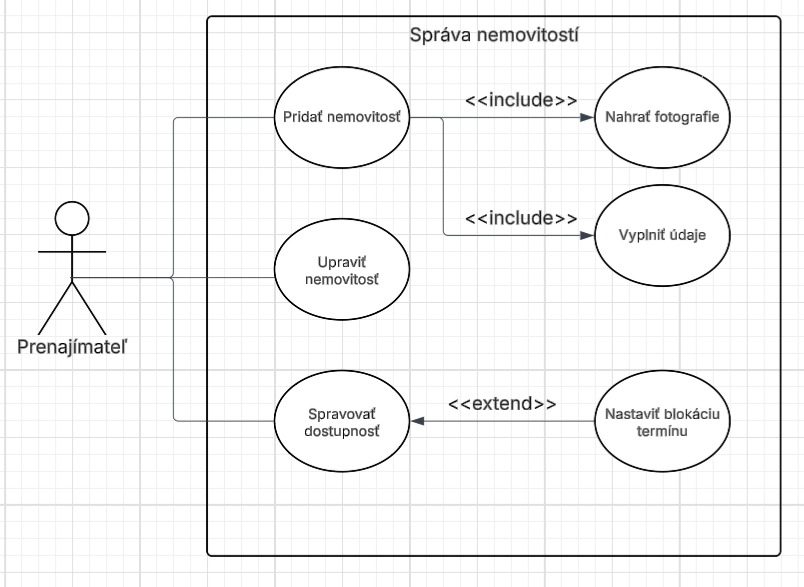
\includegraphics[width=0.92\textwidth]{usecaseNemovitosti.png}
  \caption{Use Case diagram pre správu nemovitostí -- VAL0556.}
\end{figure}

% ── UC 3: Rezervační subsystém ─────────────────────────────
\subsection{Rezervační subsystém (LIS0168)}

Diagram pokrývá celý životní cyklus rezervace. Aktéři jsou \textbf{Host} a autonomní \textbf{Časovač CRON}. Systém komunikuje s externím systémem \textbf{Platební brána}. Vazby \texttt{<<include>>} modelují povinné kroky (ověření dostupnosti, odeslání e-mailu), \texttt{<<extend>>} stornování expirované rezervace.

\begin{figure}[htbp]
  \centering
  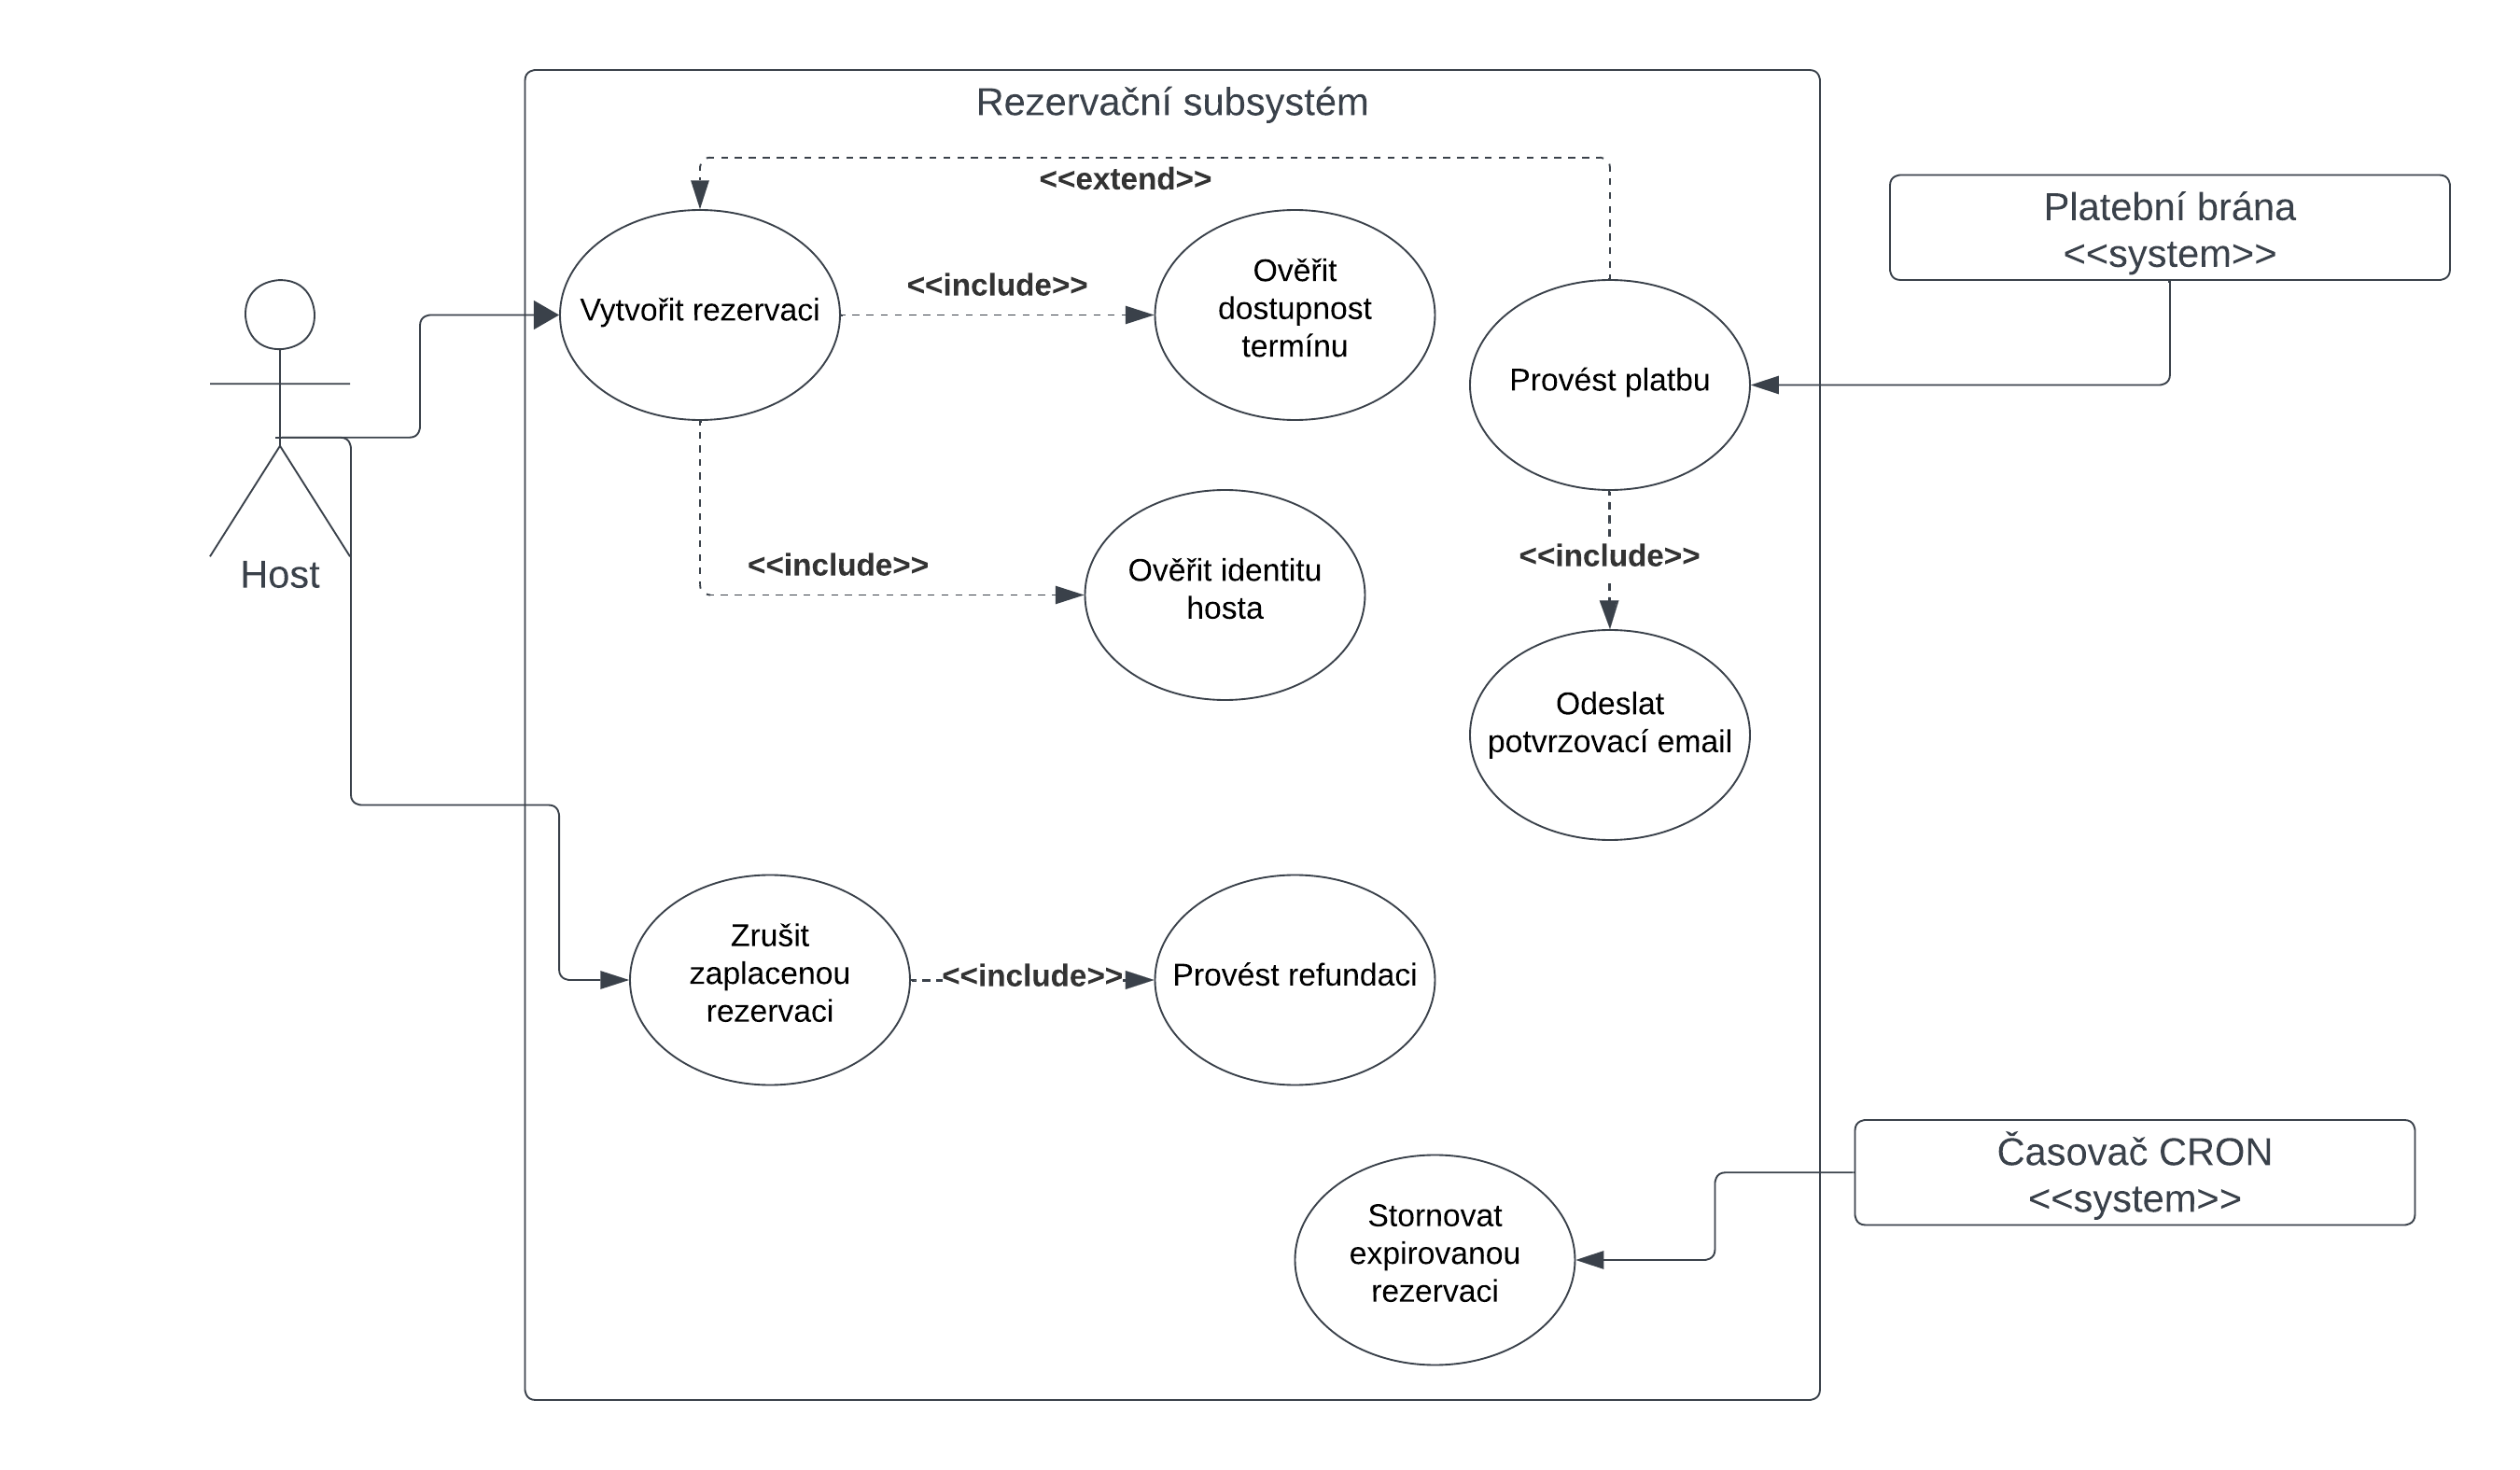
\includegraphics[width=0.92\textwidth]{usecase_rezervace.png}
  \caption{Use Case diagram pro rezervační sub-systém -- LIS0168.}
\end{figure}

\newpage

% ============================================================
\section{Scénáře (Konkrétní implementace Use Case)}
% ============================================================

% ── 10.1  NOVÉ v 0.2 ───────────────────────────────────────
\subsection{\textcolor{newblue}{Scénář: Registrácia nového užívateľa}}

{\color{newblue}
\begin{scenparams}
  \sprow{Názov}{Registrácia nového užívateľa.}
  \sprow{Kontext}{Nový záujemca o platformu (budúci Host alebo Prenajímateľ) navštívi webovú aplikáciu a chce si vytvoriť účet, aby mohol vyhľadávať ubytovanie alebo pridávať vlastné nehnuteľnosti.}
  \sprow{Level zanorenia UC}{Užívateľský cieľ.}
  \sprow{Aktéri}{Neprihlásený užívateľ (budúci Host alebo Prenajímateľ).}
  \sprow{Stakeholderi}{Zákazník/Investor (rast databázy), Administrátor (GDPR), Systém (validné identifikátory).}
  \sprow{Vstupné podmienky}{Užívateľ nie je prihlásený, má prístup k internetu a platnú e-mailovú adresu.}
  \sprow{Výstupné podmienky}{Nový záznam \textit{Uživatel} so stavom \texttt{aktivní} a zvolenou rolou; užívateľ je automaticky prihlásený.}
  \sprow{Minimálny výstup}{Záznam so stavom \texttt{neoverený} (čaká na potvrdenie e-mailu).}
  \sprow{Ideálny výstup}{Úspešná registrácia, automatické prihlásenie a presmerovanie na dashboard podľa zvolenej role.}
\end{scenparams}

\textbf{Hlavný scénár:}
\begin{enumerate}
  \item \textbf{Užívateľ} otvorí stránku a klikne na tlačidlo „Registrovať sa".
  \item \textbf{Systém} zobrazí registračný formulár (meno, priezvisko, e-mail, heslo, potvrdenie hesla, výber role).
  \item \textbf{Užívateľ} vyplní všetky povinné polia a zvolí rolu (Host\,/\,Prenajímateľ).
  \item \textbf{Užívateľ} odošle formulár kliknutím na „Vytvoriť účet".
  \item \textbf{Systém} overí formát a úplnosť polí.\\
        \textbf{Rozhodovanie:} Sú všetky polia validné? (V tomto kroku áno. Ak nie $\rightarrow$ rozšírenie 5a/5b.)
  \item \textbf{Systém} overí unikátnosť e-mailovej adresy v databáze.\\
        \textbf{Rozhodovanie:} Je e-mail unikátny? (V tomto kroku áno. Ak nie $\rightarrow$ rozšírenie 6a.)
  \item \textbf{Systém} zahashuje heslo (bcrypt) a uloží nový záznam so stavom \texttt{neoverený}.
  \item \textbf{Systém} odošle potvrdzovací odkaz cez e-mailový server (SMTP/API).\\
        \textbf{Smyčka:} Ak odkaz nebude kliknutý do 24\,h, systém odošle pripomienku (max.\ 2 pokusy). Po 48\,h bez potvrdenia systém záznam automaticky zmaže.
  \item \textbf{Užívateľ} otvorí e-mail a klikne na potvrdzovací odkaz.
  \item \textbf{Systém} zmení stav z \texttt{neoverený} na \texttt{aktivní}.
  \item \textbf{Systém} automaticky prihlási užívateľa a presmeruje ho na dashboard podľa zvolenej role.
\end{enumerate}

\textbf{Rozšírenie:}
\begin{itemize}
  \item \textbf{5a.} Neúplné polia: Systém zvýrazní chybné polia a zobrazí popis chyby. Odoslanie blokované; scenár sa vracia do kroku~3.
  \item \textbf{5b.} Heslá sa nezhodujú: Systém ihneď informuje o rozdiele. Scenár sa vracia do kroku~3.
  \item \textbf{6a.} E-mail už existuje: Systém zobrazí ponuku prihlásenia. Registrácia sa nespustí. Koniec prípadu použitia.
  \item \textbf{8a.} E-mailový server nedostupný: Systém uloží správu do fronty a opakuje odoslanie (max.\ $3\times$ s exponenciálnym oneskorením). Po neúspechu dostane upozornenie administrátor.
\end{itemize}
}% end newblue

% ── 10.2 ───────────────────────────────────────────────────
\subsection{Scénár: Vytvorenie a publikácia nového inzerátu}

\begin{scenparams}
  \sprow{Názov}{Vytvorenie a publikácia nového inzerátu nemovitosti.}
  \sprow{Kontext}{Prenajímateľ má k dispozícii voľnú nemovitosť a chce ju zaevidovať do systému, aby bola dostupná pre užívateľov.}
  \sprow{Level zanorenia UC}{Užívateľský cieľ.}
  \sprow{Aktéri}{Prenajímateľ.}
  \sprow{Stakeholderi}{Prenajímateľ (rezervácie), Systém (validné dáta), Administrátor (moderácia).}
  \sprow{Vstupné podmienky}{Prenajímateľ je prihlásený a jeho identita je overená.}
  \sprow{Výstupné podmienky}{Nemovitosť uložená v databáze, fotografie priradené, inzerát nastavený ako „Aktívny".}
  \sprow{Minimálny výstup}{Záznam uložený ako „Rozpracované".}
  \sprow{Ideálny výstup}{Úspešná validácia, uloženie a okamžitá dostupnosť nemovitosti.}
\end{scenparams}

\textbf{Hlavný scénár:}
\begin{enumerate}
  \item \textbf{Prenajímateľ} zvolí funkciu „Pridať nemovitosť" v rozhraní.
  \item \textbf{Systém} zobrazí formulár pre zadanie údajov.
  \item \textbf{Prenajímateľ} vyplní detailný formulár (názov, popis, lokalita, kapacita, cena).
  \item \textbf{Prenajímateľ} nahraje sadu fotografií.
  \item \textbf{Systém} validuje povinné polia a formát fotografií.\\
        \textcolor{newblue}{\textbf{Rozhodovanie:} Sú všetky polia správne a fotografie v požadovanom formáte? (V tomto kroku áno. Ak nie $\rightarrow$ rozšírenie 3a/4a.)}
  \item \textbf{Prenajímateľ} potvrdí uloženie.
  \item \textbf{Systém} uloží dáta do tabuliek \textit{Nemovitost} a \textit{Fotografie}.
  \item \textbf{Systém} nastaví stav na „Aktívny" a sprístupní inzerát hostom.
\end{enumerate}

\textbf{Rozšírenie:}
\begin{itemize}
  \item \textbf{3a.} Neúplné údaje: Systém zvýrazní chýbajúce pole a nepovolí uloženie. Scenár sa vracia do kroku~3.
  \item \textbf{4a.} Chybný formát fotografie: Systém vyzve k výberu iného súboru. Scenár sa vracia do kroku~4.
  \item \textbf{6a.} Prerušenie procesu: Systém uloží dáta ako „nedokončené", aby bolo možné pokračovať neskôr.
\end{itemize}

\newpage

% ── 10.3 ───────────────────────────────────────────────────
\subsection{Scénář: Vytvoření rezervace a platba}

\begin{scenparams}
  \sprow{Název}{Zpracování rezervace a úhrady ubytování.}
  \sprow{Kontext}{Host si vybral termín a klikl na „Rezervovat". Probíhá uzamčení termínu a převod peněz.}
  \sprow{Level zanoření UC}{Uživatelský cíl (Hlavní proces).}
  \sprow{Aktéři}{Host, Platební brána (externí systém).}
  \sprow{Stakeholdeři}{Pronajímatel (očekává zisk a informaci o obsazení bytu).}
  \sprow{Vstupní podmínky}{Host je autentizován; požadovaný termín je aktuálně volný.}
  \sprow{Výstupní podmínky}{Rezervace ve stavu \textit{Confirmed}, platba ve stavu \textit{Success}, termín trvale blokován v kalendáři.}
  \sprow{Minimální výstup}{Dočasný záznam v databázi se statusem \textit{Pending} (při nedokončení).}
  \sprow{Ideální výstup}{Úspěšná platba a odeslání oboustranného e-mailového potvrzení (voucheru).}
\end{scenparams}

\textbf{Hlavní scénář:}
\begin{enumerate}
  \item \textbf{Host} zadá data a potvrdí parametry rezervace.
  \item \textbf{Systém} dotáže modul správy nemovitostí a naposledy ověří dostupnost.
  \item \textbf{Systém} vytvoří záznam rezervace se stavem \textit{Pending} a aplikuje dočasný zámek termínu (15\,minut).
  \item \textbf{Systém} přesměruje relaci Hosta na \textit{Platební bránu}.
  \item \textbf{Host} (v externím rozhraní) vyplní platební údaje a potvrdí platbu.\\
        \textbf{Smyčka:} Je-li karta zamítnuta, Host může opakovat zadání, dokud nevyprší zámek termínu ($\rightarrow$ rozšíření 5a).
  \item \textbf{Platební brána} zpracuje transakci a odešle do Systému webhook o výsledku.
  \item \textbf{Rozhodování:} Je webhook úspěšný? (V tomto kroku ano.)\\
        Pokud ne $\rightarrow$ rozšíření 7a.
  \item \textbf{Systém} mění stav rezervace na \textit{Confirmed} a zámek termínu na trvalý.
  \item \textbf{Systém} volá e-mailový modul pro odeslání potvrzovacích dokladů oběma stranám.
\end{enumerate}

\textbf{Rozšíření:}
\begin{itemize}
  \item \textbf{2a.} Termín obsazen jiným uživatelem: Systém přeruší proces a zobrazí chybovou zprávu. Konec případu užití.
  \item \textbf{5a.} Karta zamítnuta: Platební brána vrací chybový kód. Cyklus se vrací do bodu~5; po vypršení zámku CRON stornuje \textit{Pending} rezervaci.
  \item \textbf{7a.} Webhook nedorazí (výpadek sítě): Systém aktivuje reconciliation job -- ručně dotáže stav transakce. Pokud potvrzena $\rightarrow$ pokračuje krokem~8. Pokud ne $\rightarrow$ stornuje rezervaci.
\end{itemize}

\end{document}
